\section{Theorie}
\label{sec:Theorie}
\subsection{Der harmonische Oszillator}
Ein harmonischer Oszillatorist ein physikalisches System, welches eine Schwingung ausführt. Das einfachste Beispiel
hierfür ist eine Feder, an welcher eine Masse  $m$ um die Ruhelage $x_0$ oszilliert.
%Abbildung einfügen
Ein harmonischer Oszillator kann dabei über die Differentailgleichung
\begin{equation}
    \ddot{x}+\omega^2\cdot x=0 \label{eqn:harmOsz}
\end{equation}
definiert werden. Im mechanischen Fall ist dabei $x$ der Ort, $\ddot{x}$ die zweite Ableitung des Ortes nach der Zeit,
also die Beschleunigung, und $\omega$ eine Konstante, welche weitere Informationen über das System, wie zum Beispiel die 
Masse $m$, ergänzt. Zudem wird sich noch zeigen, dass $\omega$ die Frequenz der Schwingung beschreibt.
\\
Die Differentailgleichung kann bei der Feder aus dem zweiten Newton'schen Axiom
\begin{equation}
    F=m\cdot\ddot{x} \label{eqn:newton2}
\end{equation} 
hergeleitet werden. Dafür wird das zweite Newton'sche Axiom der rücktreibenden Kraft der Feder gleichgesetzt. Die 
Gleichheit der beiden Kräfte folgt aus dem Reaktionsprinzip. Die rücktreibende Kraft wird bei dem obrigen Beispiel
durch das Hook'sche Gesetz beschrieben
\begin{equation}
    F=-k\cdot x \label{eqn:hook}. %Vorzeichen???
\end{equation}
Dabei ist $k$ die Federkonstante der Feder.
Durch das Gleichsetzen von \eqref{eqn:newton2} und \eqref{eqn:hook} erhält man:
\begin{equation}
    m\cdot\dddot{x}=k\cdot x \Leftrightarrow \ddot{x}+\frac{k}{m}\cdot x=0 \label{eqn:dgl}
\end{equation}
Gesucht ist nun die Funktion $x(t)$, die die Differentailgleichung löst. Man wählt nun den Ansatz:
\begin{align}
    x(t)&=A\cdot cos(\omega\cdot t)+B\cdot sin(\omega\cdot t) \\
    \ddot{x}(t)&=-\omega^2\cdot x(t)
    \label{eqn:ansatz}
\end{align}
$A$ und $B$ sind dabei Konstanten, die durch die Anfangsbedingung bestimmt werden. Einsetzen des Ansatzes \eqref{eqn:ansatz}
in die Differentailgleichung \eqref{eqn:dgl} ergibt dann:
\begin{equation}
    A\cdot cos(\omega\cdot t)+B\cdot sin(\omega\cdot t)(\frac{k}{m}-\omega^2)=0
\end{equation}
Da der erste Fraktor der Gleichung nicht für alle Zeiten $t=0$ sein kann, muss der zweite Faktor null ergeben
\begin{equation}
    \frac{k}{m}-\omega^2=0 \Leftrightarrow \frac{k}{m}=\omega^2 .
\end{equation}
Aus dem Ansatz \eqref{eqn:ansatz} wird nun auch ersichtlich, dass $\omega$ die Frequenz der Schwingung beschreibt. Dies erfolgt 
unter anderem aus der Überlegung, dass das Produkt innherhalb des Sinus einheitenlos sein muss. Da die Zeit $t$ in Sekunden gegeben
ist, muss $\omega$ die Einheit $[\omega]=s^{-1}$ besitzen, also die Einheit einer Frequenz.
Die Schwingungsdauer $T$ des Pendles kann nun aus der Frequenz $\omega$ berechnet werden mit:
\begin{equation}
    T=\frac{2\pi}{\omega}
\end{equation}

\subsection{Das mathematische Pendel}
Auch ein mathematisches Pendel ist für kleine Auslenkungen näherungsweise ein harmonischer Oszillator. Das Pendel soll dabei eine
Punktmasse $m$ am Ende eines massenlosen Fadens sein, welcher eine konstatnte Länge $l$ hat und reibungsfrei hin und her schwingen kann.
Die Differentailgleichung erlangt man wieder durch das gleichsetzen von \eqref{eqn:newton2} und der rücktreibenden Kraft des Systems.
Diese ist nun aber:
\begin{equation}
    F_\text{rück}=-m\cdot g\cdot sin(\phi(t)) \label{eqn:pendelkraft}
\end{equation}
In \eqref{eqn:newton2} müssen wir jetzt noch die Beschleunigung $\ddot x$ an das Prolem anpassen. Diese ist bei einem Pendel die tangentiale
Beschleunigung. Es gilt:
\begin{equation}
    \ddot x(t)=l\cdot \ddot{\phi}(t)
\end{equation}
Der Winkel $\phi(t)$ beschreibt dabei die Auslenkung des Pendels zum Zeitpunkt $t$. Durch Gleihsetzen von \eqref{eqn:newton2} und 
\eqref{eqn:pendelkraft} erhält man nun die Differentailgleichung
\begin{eqnarray}
    \ddot{\phi}(t)+\frac{g}{l}sin(\phi(t))=0.
\end{eqnarray}
Die Differentailgleichung ist auf Grund des Sinus jedoch nicht linear, und deswegen weder analytisch lösbar, noch ein harmonischer Oszillator.
Um die Differentailgleichung trotzdem lösen zu können, betrachten wir die Taylorfunktion des Sinus:
\begin{equation}
    sin(x)=\sum_{n=0}^\infty (-1)^n\frac{x^{2n+1}}{(2n+1)!}
\end{equation}
Für $n=0$ ergibt sich die sogenannte Kleinwinkelnäherung
\begin{equation}
    sin(x)\approx x.
\end{equation}
Durch diese erlangt man zumindest für kleine Winkel $\phi$ eine lineare Differentailgleichung der Form \eqref{eqn:harmOsz}. Zwar macht man bei der 
Kleinwinkelnäherung einen Fehler, dieser ist für kleine Winkel jedoch so gering, dass wir die Näherung für die weiteren Berechnungen verwenden.
Dies bedeutet aber auch, dass im Folgenden nurnoch von kleinen AUslenkungen des Pendels ausgegangen wird!
\\
Die Differentailgleichung lautet nun
\begin{equation}
    \ddot{\phi}(t)+\frac{g}{l}\phi(t)=0
\end{equation}
und wird durch den Ansatz \eqref{eqn:ansatz} gelöst. Die Frequenz ergibt sich dabei zu
\begin{equation}
    \omega=\sqrt{\frac{g}{l}}.
\end{equation}
Die Frequenz des Pendels ist also sowohl unabhängig von der Masse $m$, als auch von der Auslenkung, solange diese hinreichend klein ist.

\subsection{Das physikalische Pendel}
Anders als bei dem mathematischen Pendel ist die Masse des physikalischen Pendels nicht in einem Punkt am Ende eines massenlosen Fadens komprimiert.
Das Pendel hat nun auf der gesamten Länge eine Masse und kann beliebig geformt sein. Um die zusätzlichen Informationen in die Differentailgleichung
zu integrieren, führt man die Größe des Trägheitsmoments $J$ ein. Dieses ist definiert als:
\begin{equation}
    J=\rho\int{\vec{r}^2\rho(\vec{r})dV}
\end{equation}
Dabei ist $\rho$ die Dichte des Körpers an der jeweiligen Stelle.
\\
Die Differentailgleichung des Pendles wird dadurch zu:
\begin{equation}
    \ddot{\phi}+\frac{mgl}{J}=0
\end{equation}
Die Frequenz ändert sich zu:
\begin{equation}
    \omega=\frac{mgl}{J}
\end{equation}

\subsection{Gekoppelte Pendel}
Koppelt man zwei identische Pendel mit einer Feder, so schwingen diese nicht mehr unabhängig von einander, da die Pendel zusätzliche Kräfte auf 
einander auswirken. Als zusätzlichen Größen erhält man die Federkonstatnt $k$. Zudem sind nun zwei Längen für das System relevant, nämlich die 
Länge der Pendel $L$ und der Abstand $l$ an dem die Feder an den Pendeln befestigt ist. 
\\
Man erhält nun ein Systemaus zwei Differentailgleichungen, die zudem mit einander gekoppelt sind:
\begin{align}
    J\ddot{\phi}_1&=-mgl\phi_1+kl^2(\phi_2-\phi_1)\\
    J\ddot{\phi}_2&=-mgl\phi_2+kl^2(\phi_2-\phi_1)
\end{align}
Das Differentailgleichung-System wird im Folgenden nur für drei verschiedene Anfangsbedingungen gelöst, da nur diese für den Versuch relevant sind.
Die Anfangsbedingungen sind hierbei die Winkel $\alpha_1$ und $\alpha_2$ mit denen die Pendel zu Beginn ausgelenkt werden, und die Geschwindigkeiten
$v_1$ und $v_2$, die die Pendel zu Beginn erhalten. Für die drei relevanten Fälle gilt: $v_1=v_2=0$

\begin{enumerate}
    \item Gleichsinnige Schwingung: $\alpha_1=\alpha_2$
        \begin{figure}
        \centering
        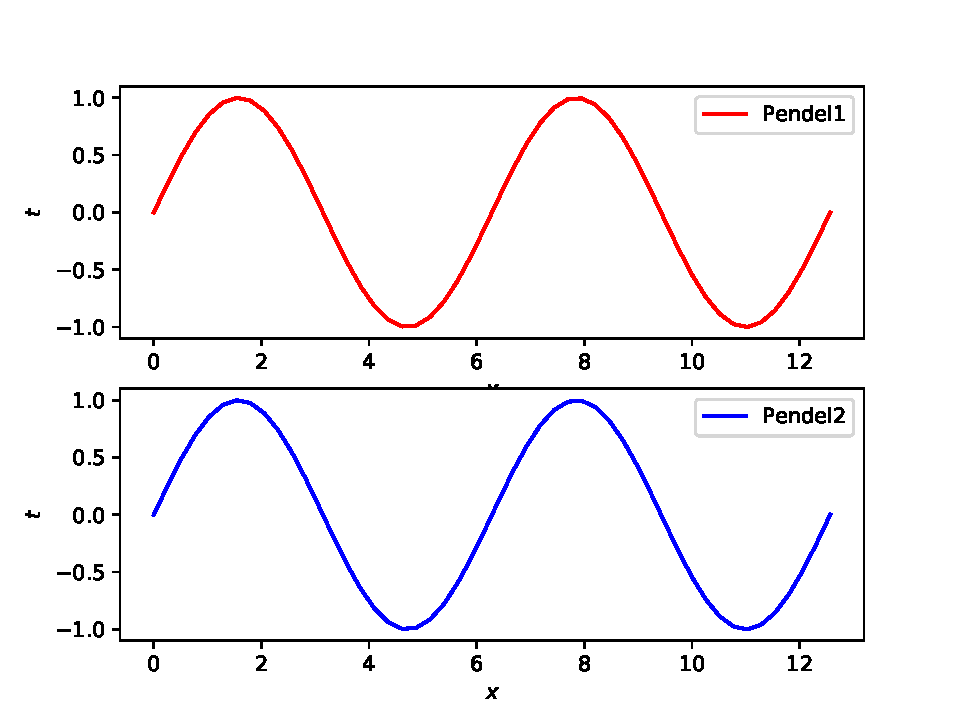
\includegraphics[scale = 0.5]{gleichsinnig.pdf}
        \caption{Amplituden in Abhängigkeit von t bei gleichsinniger Schwingung}
        \label{fig:gleichsinnig}
      \end{figure}
    \item Gegensinnige Schwingung: $\alpha_1=-\alpha_2$
    \begin{figure}
        \centering
        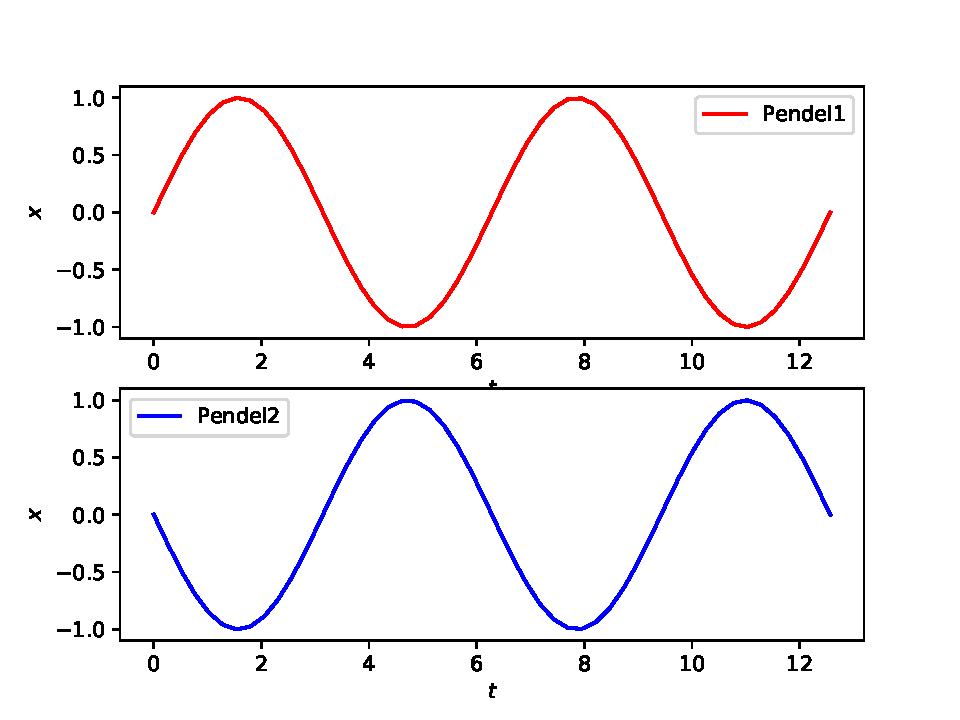
\includegraphics[scale = 0.5]{gegensinnig.pdf}
        \caption{Amplituden in Abhängigkeit von t bei gegensinniger Schwingung}
        \label{fig:gegensinnig}
      \end{figure}
    \item Gekoppelte Schwingung: $\alpha_1=0$, $\alpha_2\neq 0$
    \begin{figure}
        \centering
        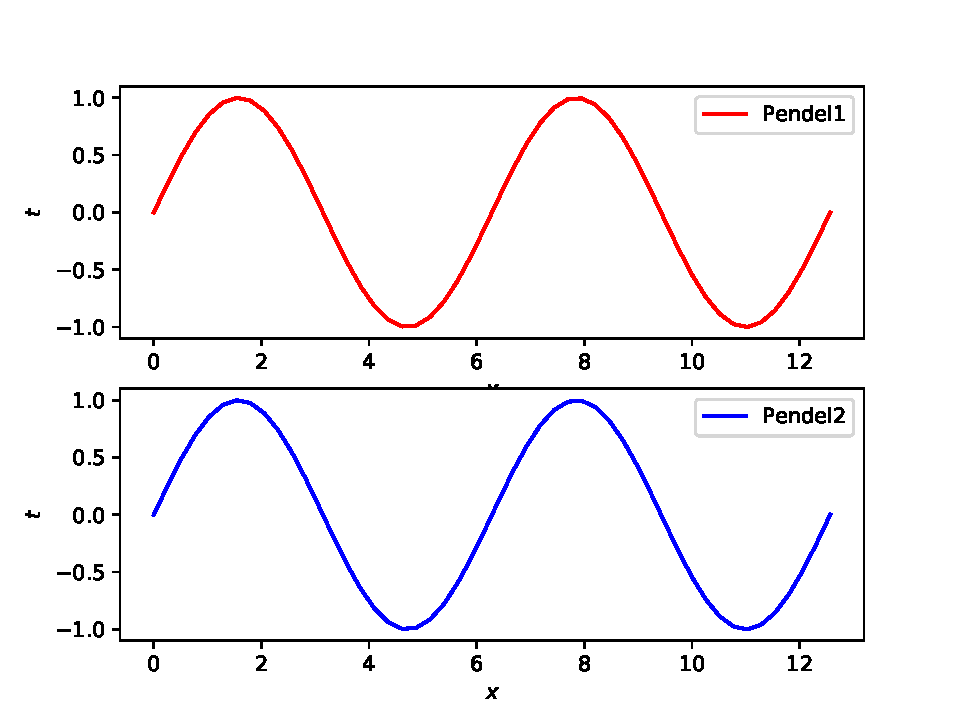
\includegraphics[scale = 0.5]{gleichsinnig.pdf}
        \caption{Amplituden in Abhängigkeit von t bei gekoppelter Schwingung}
        \label{fig:gleichsinnig}
      \end{figure}
\end{enumerate}